\documentclass{article}
\usepackage[left=8em,right=8em]{geometry}
\usepackage{amsmath,amsthm,amssymb}
\usepackage{lineno}
\usepackage{relsize}
\usepackage{graphicx}
\usepackage{hyperref}

\hypersetup{
    colorlinks=true,
    linkcolor=blue,
}
%\linenumbers
\renewcommand*{\proofname}{Proof}
\date{}
\author{}
\begin{document}
\centerline{\textbf{Exercises for Section 11.5}}
$ $\newline
\textbf{Ex 1.} Addition and multiplication tables for $\mathbb{Z}_2$
\begin{figure}[h]
\centering
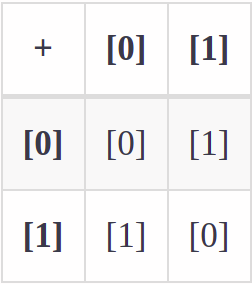
\includegraphics[scale=0.5]{11_5_1a.png}
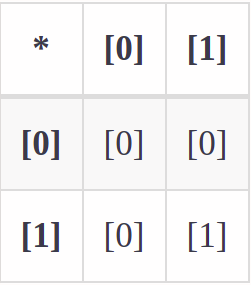
\includegraphics[scale=0.5]{11_5_1b.png}
\end{figure}\\
\textbf{Ex 2.} Addition and multiplication tables for $\mathbb{Z}_3$
\begin{figure}[h]
\centering
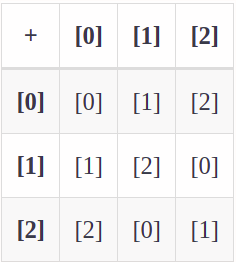
\includegraphics[scale=0.66]{11_5_2a.png}
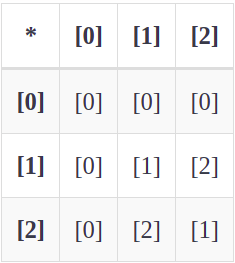
\includegraphics[scale=0.66]{11_5_2b.png}
\end{figure}\\
\newpage
\noindent\textbf{Ex 3.} Addition and multiplication tables for $\mathbb{Z}_4$
\begin{figure}[h]
\centering
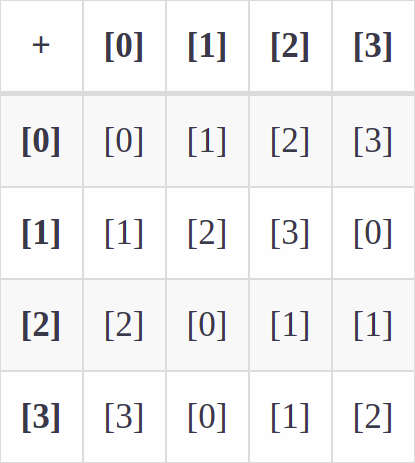
\includegraphics[scale=0.5]{11_5_3a.png}
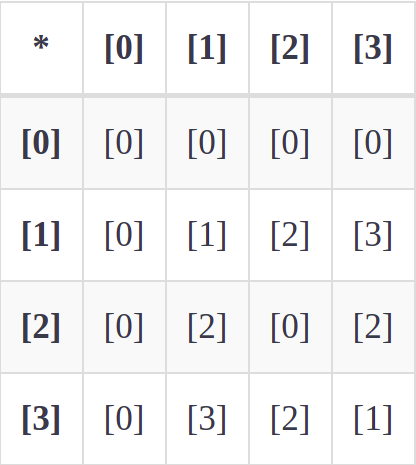
\includegraphics[scale=0.5]{11_5_3b.png}
\end{figure}\\
\newpage
\noindent\textbf{Ex 4.} Addition and multiplication tables for $\mathbb{Z}_6$
\begin{figure}[h]
\centering
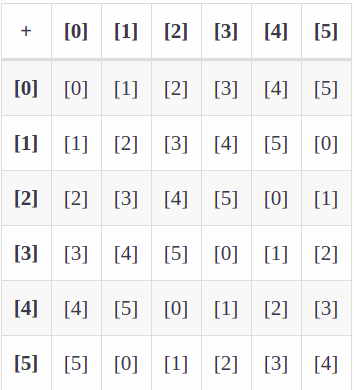
\includegraphics[scale=0.6]{11_5_4a.png}

\includegraphics[scale=0.6]{11_5_4b.png}
\end{figure}\\
\noindent\textbf{Ex 5.Proposition:} If $[a],[b] \in \mathbb{Z}_5$ and $[a] \cdot{} [b] = [0]$, then $[a]=[0]$ or $[b] = [0]$.
\begin{proof}
(Contradiction.) Suppose $[a],[b] \in \mathbb{Z}_5$, $[a] \cdot{} [b] = [0]$, $[a] \neq [0]$, and $[b] \neq [0]$.\\
$[a] \neq [0]$ implies that $a = 5x+r$ for some integers $x, r$ where $1 \leq r \leq 4$. Likewise, $[b] \neq [0]$ implies that $b=5y+c$ for some integers $y, c$ where $1 \leq c \leq 4$. Then $[a] \cdot{} [b] = [0]$ implies that $5$ divides $a \cdot{} b = (5x+r)(5y+c)=25xy+5xc+5yr+cr$. Thus $cr$ must be divisable by $5$. But this contradicts Euclid's lemma. Therefore it must be the case that $[a]=[0]$ or $[b]=[0]$.\\ 
\end{proof}
\noindent\textbf{Ex 6.} For $\mathbb{Z}_6$, note the counter-example for $\mathbb{Z}_6$: $[2] \cdot{} [3] = [2 \cdot{} 3] = [6] = [0]$. For $\mathbb{Z}_7$, the statement is true. A proof almost identical to the one above could be used to show the statement to be true.\\

\noindent\textbf{Ex 7.}\\
a) $[8]+[8]=[8+8]=[16]=[7]$\\
b) $[24]+[11]=[24+11]=[35]=[8]$\\
c) $[21] \cdot{} [15] = [21 \cdot{} 15]= [315]=[0]$\\
d) $[8] \cdot{} [8] = [8 \cdot{} 8] = [64] = [1]$\\

\noindent\textbf{Ex 8. Proposition:} If $[a], [b] \in \mathbb{Z}_n$, $[a] = [a']$, and $[b] = [b']$, then $[a] + [b] = [a'] + [b']$.
\begin{proof}
(Direct). Suppose $[a], [b] \in \mathbb{Z}_n$, $[a] = [a']$, and $[b] = [b']$.\\
Because $[a]=[a']$, it follows that $n$ divides $a-a'$, so $a-a'=nx$ for some integer $x$. Likewise, $[b]=[b']$ implies that $n$ divides $b-b'$, so $b-b'=ny$ for some integer $y$. Then $a+b=(nx+a')+(ny+b') \leftrightarrow (a+b) - (a'+b')= n(x+y) \leftrightarrow a+b \equiv a'+b' \pmod{n}$. Therefore $[a] + [b] = [a'] + [b']$.\\
\end{proof}

\end{document}

